\subsection{Test Model}

To simplify our verification, we only use a rather small CNN model on MNIST dataset. This CNN model is based on the classical LeNet-5 with BN but without implicit linear layer. The model can achieve a 98\% Acc. easily.

\begin{figure}[!htb]
    \centering
    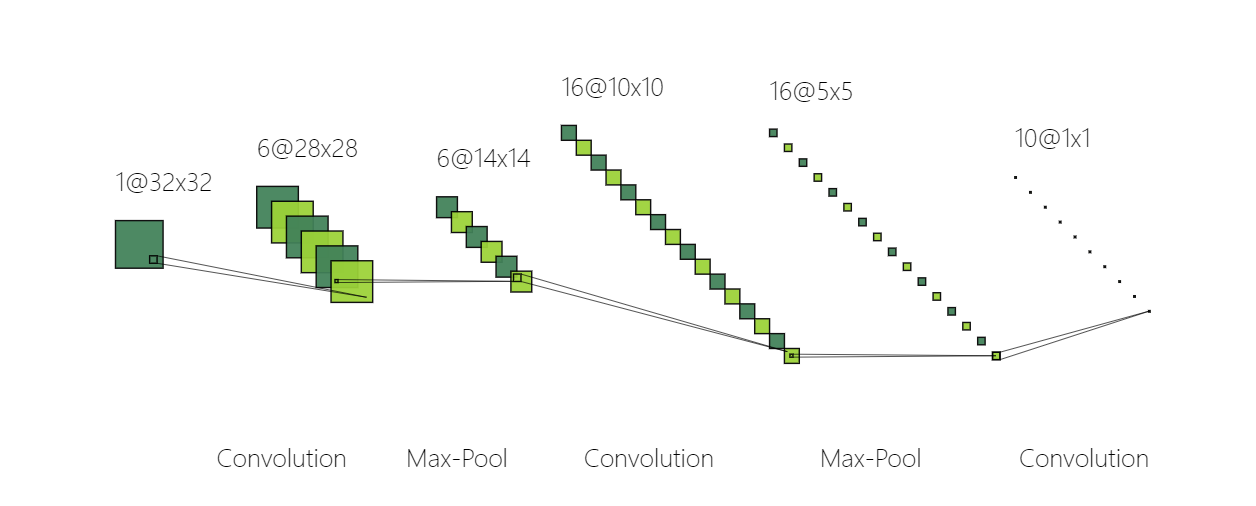
\includegraphics[width=\columnwidth]{../figures/net.png}
    \caption{Out test model}
    \label{fig:net}
\end{figure}

After each convolution layer, we apply a ReLU and BN.

Then we analyze the distribution of parameters and pixels under inference.

\begin{figure}[!htb]
    \centering
    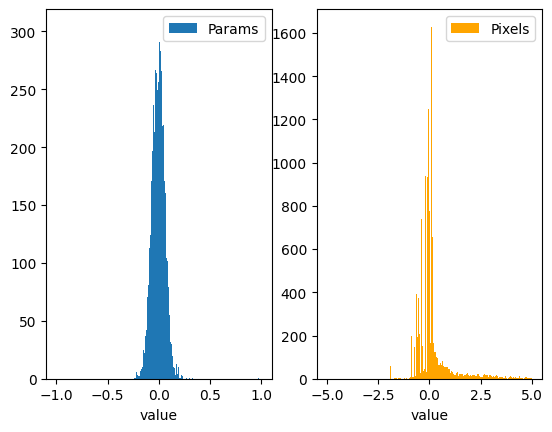
\includegraphics[width=0.9\columnwidth]{../figures/distribution.png}
    \caption{Distribution of parameters and pixels}
    \label{fig:distribution}
\end{figure}

As \figref{fig:distribution} shows, parameters has a much smaller variation, with most value inside $(-0.25, 0.25)$, and the mean value is about 0. But the distribution of pixels is much more complicated. Due to ReLU, most negatives are clamped to 0. At the same time, the variation is larger, with noticeable number of pixels extended to positive 5, actually the biggest value can reach more than 20 during inference, causing the fixed point setting difficult and tricky.